
%----------------------------------------------------------------------------------------%
% START LaTeX preamble

% define document type, font and paper size
\documentclass[11pt,a4paper]{article}

%----------------------------------------------------------------------------------------%
% IMPORT LaTeX packages

\usepackage{inputenc}
\usepackage[ngerman, english]{babel}
\usepackage{csquotes}
\usepackage{amsmath}
\usepackage{amssymb}
\usepackage{amsfonts}
\usepackage{graphicx}
\usepackage{wrapfig}
\usepackage[margin=1.25in]{geometry}
\usepackage{pdfpages}
\usepackage{listings}
\usepackage{setspace}
\usepackage{systeme}
\usepackage{mdframed}

%----------------------------------------------------------------------------------------%
% SET user defined commands

\newcommand{\mathsym}[1]{{}}
\newcommand{\unicode}[1]{{}}

%----------------------------------------------------------------------------------------%
% IMPORT LaTeX packages to manange bibliography

% MLA, APA, or IEEE? - https://www.overleaf.com/learn/latex/Biblatex_citation_styles
\usepackage[style=apa]{biblatex}
\addbibresource{bibliography.bib}

%----------------------------------------------------------------------------------------%
% DEFINE header values

% define the cover page values
\title
{
    Thesis Message\\
    Carbon nano-wires synthesis through electrospun-able, photopolymerizable and pyrolyzable/graphitizable fibers
}
\author
{
    Antonio Osamu Katagiri Tanaka \\
    A01212611
}
\date{\today}

%----------------------------------------------------------------------------------------%
% USER-DEFINED commands

% Keywords command
\providecommand{\keywords}[1]
{
    \\
    \\
    \small
    \textbf{\textit{Keywords:}} #1
}

%----------------------------------------------------------------------------------------%

\begin{document}

%----------------------------------------------------------------------------------------%
% CREATE the 1st page (cover page)

\maketitle

%----------------------------------------------------------------------------------------%
% DEFINE the abstract text & keywords

%\begin{abstract}
%    \emph
%    {
%        Lorem ipsum dolor sit amet, consectetur adipiscing elit, sed do eiusmod tempor incididunt ut labore et dolore magna aliqua. Ut enim ad minim veniam, quis nostrud exercitation ullamco laboris nisi ut aliquip ex ea commodo consequat. Duis aute irure dolor in reprehenderit in voluptate velit esse cillum dolore eu fugiat nulla pariatur. Excepteur sint occaecat cupidatat non proident, sunt in culpa qui officia deserunt mollit anim id est laborum.
%    }
%    \keywords{Lorem, ipsum, dolor, sit, amet}
%\end{abstract}

%----------------------------------------------------------------------------------------%

\begin{enumerate}
  \item {Carbon fibers are versatile materials composed of carbon chains with a wide range of applications.}
  \item {Carbon nanowires have been fabricated with a photoresist, but little is known about polymers that can produce more conductive carbon nanowires after pyrolysis.}
  \item {FFES or Far field electrospinning is a inexpensive process to produce polymer fibers, but with low accuracy due to electric instabilities.}
  \item {Near field electrospinning (NFES) is similar to FFES, but with a reduced distance between the fiber source and the collector and higher precision.}
  \item {Various polymer solutions have being tested and measured through NFSE and photopolymerization processes; it was found that it is not possible to predict the behaviour of the electrospinning process, so additional properties are to be considered to achieve a stable process.}
  \item {The properties of the polymer solution can be amended to obtain a electrospun-able, photopolymerizable and pyrolyzable/graphitizable fibers.}
  \item {Analyse the rheology of different polymer solutions to determine if they can be easily electrospun at low voltages and then fabricate nanowires with them.}
  \item {Design polymer solutions that can be electrospun by NFES, photopolymerized, and then pyrolyzed into conducting carbon nanowires.}
  \item {The use of the newly designed polymer solution within the NFES-Photopolymerization-Pyrolysis process can be amended to achieve mass scale manufacturing of carbon nanowires in a cheap, continuous, simple and reproducible manner.}
  \item {The new/tailored polymer solution can be used to synthesize carbon nanowires with high conductive properties and reduced thickness.}
\end{enumerate}

\clearpage

%----------------------------------------------------------------------------------------%
% CREATE a table of contents in a new page

%\tableofcontents
%\clearpage

%----------------------------------------------------------------------------------------%
% CREATE a list of figures and a list of tables in a new page

%\listoffigures
%\listoftables
%\clearpage

%----------------------------------------------------------------------------------------%
% DOCUMENT body starts here


%----------------------------------------------------------------------------------------%
% PRINT bibliography/references in a new page

\clearpage
\printbibliography

%----------------------------------------------------------------------------------------%
% ADD appendixes
\appendix % headings numbered with letters

%----------------------------------------------------------------------------------------%
% APPEND instructions
%\section{Assessment Instructions}\label{sec:instructions}
%[Refer to the next page]

%
\includepdf[page=-]{pdf/MII-AssessedExercise02-201911}

%----------------------------------------------------------------------------------------%
% APPEND registration
%\section{49CIDTEC registration}\label{sec:registration}
%[Refer to the next page]

%Notice that only the pre-registration is included, as all the sessions were attended %remotely from \emph{Tecnológico de Monterrey} - \emph{Campus Estado de México}.

%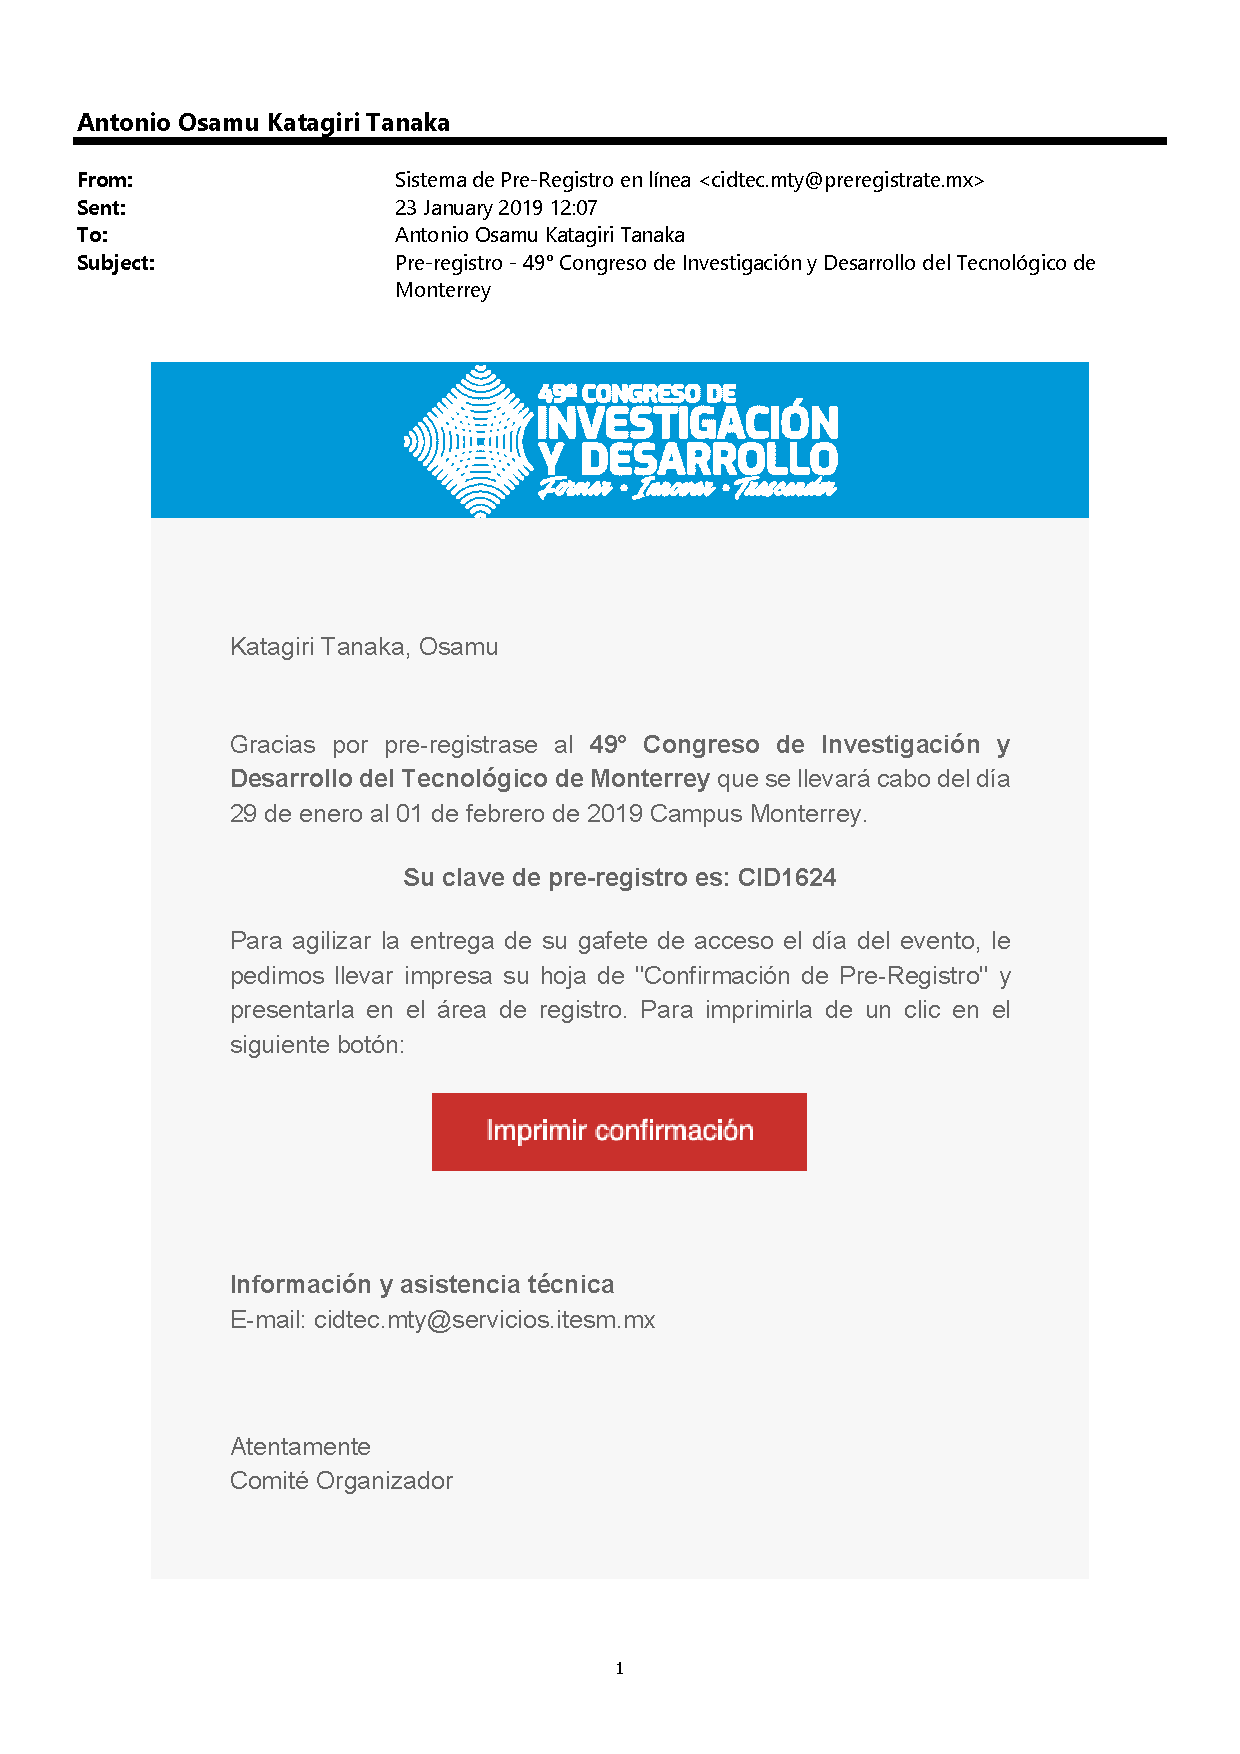
\includepdf[page=-]{pdf/49CIDTEC_preregistro}

%----------------------------------------------------------------------------------------%

\end{document}

%----------------------------------------------------------------------------------------%
